% Slides accompanying "Learn RISC-V CPU Implementation and BSV" book
% Copyright (c) 2024 Rishiyur S. Nikhil, All Rights Reserved

% -*- mode: fundamental -*-

% Slides accompanying "Learn RISC-V CPU Implementation and BSV" book
% Copyright (c) 2024 Rishiyur S. Nikhil, All Rights Reserved

% This is a preamble shared by all the slide decks

\documentclass[10pt, aspectratio=169]{beamer}

% \documentclass[17pt]{beamer}

% Avail. font sizes: 8pt, 9pt, 10pt, 11pt, 12pt, 14pt, 17pt, 20pt.
% Default font size is 11pt (= 22pt in full screen mode).

\usepackage{verbatim}
\usepackage{fancyvrb}
\usepackage{listings}

\usepackage{array}

% ================================================================
% Themes

\usetheme{Madrid}          % Line at bottom: Author (affiliation), OptTitle, Conf, page 

% \usetheme{Copenhagen}    % Same as Madrid except bottom line: Author, OptTitle

% \usetheme{Berkeley}    % Takes up 1-inch border on left and top

% ----------------
% colorthemes
% (default), beaver, beetle, seahorse, wolverine

\usecolortheme{seahorse}

% ================================================================
% Customization: show table of contents before each section
% Use \AtBeginSubsection    to show before each subsection

% \AtBeginSection[]
% {
%   \begin{frame}
%     \frametitle{Table of Contents}
%     \tableofcontents[currentsection]
%   \end{frame}
% }

% ================================================================

% ----------------
% The bsc compiler and BSV language
\newcommand{\bsc}{\emph{bsc}}
\newcommand{\BSV}{\bf{BSV}}
% ----------------
% ITALICISE WORDS
\newcommand{\ie}{\emph{i.e.,}}
\newcommand{\eg}{\emph{e.g.,}}
\newcommand{\Eg}{\emph{E.g.,}}
\newcommand{\etc}{\emph{etc.}}
\newcommand{\via}{\emph{via}}
\newcommand{\vs}{\emph{vs.}}

% ----------------
% EMPTY BOXES OF VARIOUS WIDTHS, FOR INDENTATION (N 'em' spaces)

\newcommand{\hm}{\hspace*{1em}}
\newcommand{\hmm}{\hspace*{2em}}
\newcommand{\hmmm}{\hspace*{3em}}
\newcommand{\hmmmm}{\hspace*{4em}}

% ----------------
% Convenient widths (less than text width by N 'em' spaces)

\newlength{\hlessmm}
\setlength{\hlessmm}{\textwidth}
\addtolength{\hlessmm}{-2em}

\newlength{\hlessmmm}
\setlength{\hlessmmm}{\textwidth}
\addtolength{\hlessmmm}{-3em}

\newlength{\hlessmmmm}
\setlength{\hlessmmmm}{\textwidth}
\addtolength{\hlessmmmm}{-4em}

% ----------------
% EMPTY LINES of various heights  (N 'ex' heights)

\newcommand{\vx}{\vspace*{1ex}}
\newcommand{\vxx}{\vspace*{2ex}}
\newcommand{\vxxx}{\cspace*{3ex}}
\newcommand{\vxxxx}{\vspace*{4ex}}

% ----------------
% Inputting verbatim code fragments, with various font sizes

\newcommand{\SHOWCODE}[1]{{\footnotesize\input{#1}}}

\newcommand{\SHOWCODESCRIPT}[1]{{\scriptsize\input{#1}}}

\newcommand{\SHOWCODETINY}[1]{{\tiny\input{#1}}}

% ----------------
% To allow redefinition of "pause" during development vs. deployment
% Argument is vertical space command

% Choose with or without pauses
% \newcommand{\PAUSE}[1]{#1\pause}
\newcommand{\PAUSE}[1]{#1}

% ----------------
% Emojis

\graphicspath{ {./../Figures/} }

\newcommand{\EmojiExercise}{\begin{minipage}[c]{5em}
  \includegraphics[width=3em]
    {person-lifting-weights-emoji-clipart-md-3307277008.png}
\end{minipage}}

% ================================================================
% Title page

\title[Learn CPU design \& {\BSV}]{Learn RISC-V CPU Implementation and {\BSV}}

\subtitle{({\BSV}: a High-Level Hardware Design Language)}

\author[{\copyright} R.S.Nikhil]{Rishiyur S.~Nikhil}
% \institute{Bluespec, Inc.}

% Date is set differently in each slide deck

% \logo{\includegraphics[height=0.6cm]{../Figures/Bluespec_Logo_2022-10}}

% End of preamble
% ****************************************************************


\date{L11: {\BSV}: Verifiying BSV Designs}

% ****************************************************************

\begin{document}

% ================================================================

\begin{frame}
\titlepage

\begin{center}
 \includegraphics[height=1cm]{Bluespec_Logo_2022-10}
\end{center}

\end{frame}

% ================================================================

\section{Reminders}

% -*- mode: fundamental -*-

% ================================================================

\begin{frame}[fragile]
\frametitle{Reminders}

\footnotesize

Please git clone: \url{https://github.com/rsnikhil/Learn_Bluespec_and_RISCV_Design} \\
(git pull for latest version).  Repsitory structure:

\vspace{1ex}

\begin{minipage}{0.5\textwidth}\scriptsize
\begin{Verbatim}[frame=single, numbers=left]
    ./Book_BLang_RISCV.pdf
      Slides/
          Slides_01_Intro.pdf
          Slides_02_ISA.pdf
          ...
      Exercises/
          Ex-03-A-Hello-World/
          Ex-03-B-Top-and-DUT/
          ...
      Code/
          src_Top/
          src_Drum/
          src_Fife/
          src_Common/
          ...
      Doc/Installing_bsc_Verilator_etc.{adoc,html}
\end{Verbatim}
\end{minipage}
\hm
\begin{minipage}{0.45\textwidth}
\begin{itemize}

 \item Slides and Exercise are numbered in sync with book Chapter numbers.

 \item For Exercises, please see Appendix E of the book.  Some (not
       all) exercises have associated code in the {\tt Exercises/}
       directory.

\end{itemize}
\end{minipage}

\vspace{2ex}

To compile and run the code for exercises, Drum and Fife, please make sure you have installed:

\begin{itemize}

 \item \emph{bsc} compiler (see \url{https://github.com/B-Lang-org/bsc})

 \item Verilator compiler (see \url{https://www.verilator.org/})
\end{itemize}

\footnotesize

\end{frame}

% ================================================================

\begin{frame}
\frametitle{Chapter Roadmap}

\footnotesize

\begin{center}
\frame{\includegraphics[height=0.825\textheight]{Fig_Chapter_Roadmap}}
\end{center}

\end{frame}

% ================================================================


% ================================================================

\begin{frame}
\frametitle{Table of Contents}

\tableofcontents

\end{frame}

% ****************************************************************

\section{Testbenches and DUTs}

\begin{frame}

\begin{center}
  {\LARGE {\BSV}: Testbenches and DUTs}
\end{center}

\end{frame}

% ================================================================

\begin{frame}[fragile]
\frametitle{Typical verification system setup}

\footnotesize

\begin{minipage}{0.59\textwidth}
 \includegraphics[width=\textwidth]{Fig_Testbench_DUT}
\end{minipage}
\hfill
\begin{minipage}{0.4\textwidth}

{\tt mkTop} has {\tt Empty} interface and merely serves to intantiate
and connect:

\begin{itemize}
    \item DUT = ``Design Under Test''

    \item Testbench \\
        (Tb, Test Harness, Test Environment)

        \vx
        Contains:
        \begin{itemize}\scriptsize
            \item Stimulus generator: provides inputs to DUT (via DUT methods)

            \vx
            \item Result logger/checker: collects outputs from DUT
                (via DUT methods), and records/analyzes/checks them.

        \end{itemize}

\end{itemize}

\end{minipage}

\begin{itemize}
    \item Testbenches can be written in SystemVerilog ({\eg}, UVM, simulation only).

    \item Testbenches can import C code to read/write files, run
        generator and analysis programs, {\etc} (simulation only).

    \item Testbenches may be \emph{synthesizable}, in which case the
        whole setup can run on FPGAs.

\end{itemize}

\end{frame}

% ****************************************************************

\section{{\bf printf}-style debugging}

\begin{frame}

\begin{center}
  {\LARGE {\BSV}: {\bf printf}-style debugging}
\end{center}

\end{frame}

% ================================================================

\begin{frame}[fragile]
\frametitle{{\bf printf}-style debugging}

\footnotesize

{\BSV} has the same print-like statements as Verilog and SystemVerilog:

\vx

\hmmmm
\begin{minipage}{0.7\textwidth}\tt
\begin{tabbing}
\hmmm\= \$fdisplay \= ( {\it file}, \= {\it format-string}, {\it arg}, ..., {\it arg} ) \kill
     \> \$write    \> (             \> {\it format-string}, {\it arg}, ..., {\it arg} ) \\
     \> \$display  \> (             \> {\it format-string}, {\it arg}, ..., {\it arg} ) \\
\\
     \> {\it file} <- \$fopen ("log.txt", "w"); \\
     \> ... \\
     \> \$fwrite   \> ( {\it file}, \> {\it format-string}, {\it arg}, ..., {\it arg} ) \\
     \> \$fdisplay \> ( {\it file}, \= {\it format-string}, {\it arg}, ..., {\it arg} )
\end{tabbing}
\end{minipage}

\PAUSE{\vxx}

\begin{itemize}

    \item The first two write to ``standard output'' ({\ie} the
        terminal); the latter two to a file.  All are relevant only in
        simulation; no hardware is generated for any of them.

    \vx
    \item
    {\tt \$write} and {\tt \$fwrite} do not append a trailing newline to the output;
    {\tt \$display} and {\tt \$fdisplay} do.

    \vx
    \item
    The format string is a string (in double-quotes) with formatting
    directives for the arguments that follow (\verb|%d| for signed
    integers, \verb|%b| for binary numbers, \verb|%h| for hexadecimal
    numbers, {\etc}).

    \vx
    \item In BSV, additionally, you can interleave format strings and
        arguments, like this:

    \hmmmm
    \$display  ({\it format-string}, {\it arg}, ..., {\it format-string}, {\it arg}, ... )

\end{itemize}

\end{frame}

% ================================================================

\subsection{Formatted strings}

% ================================================================

\begin{frame}[fragile]
\frametitle{Formatted strings (of type {\tt Fmt})}

\footnotesize

In {\BSV}, arguments in {\tt \$write} and {\tt \$display} statements
can also be value of type ``{\tt Fmt}'', representing a formatted
string.

\vx

For many struct and enum definitions, we append a ``{\tt deriving
(FShow)}'' clause, like this:

\vx

\begin{center}
\begin{minipage}{0.4\textwidth}
\begin{Verbatim}[frame=single]
typedef enum {OPCLASS_SYSTEM,
              ...}
OpClass
deriving (Bits, Eq, FShow);
\end{Verbatim}
\end{minipage}
\hmmmm
\begin{minipage}{0.4\textwidth}
\begin{Verbatim}[frame=single]
typedef struct {
    ...
} Decode_to_RR
deriving (Bits, FShow);
\end{Verbatim}
\end{minipage}
\end{center}

\PAUSE{\vx}

Consequently, the {\bsc} compiler automatically defines a function
{\tt fshow()} that takes an argument of that type and returns a
``formatted string'' of type {\tt Fmt}, which can be used in a
{\tt \$display()}, like this:

\vx

\begin{center}
\begin{minipage}{0.4\textwidth}
\begin{Verbatim}[frame=single]
   OpClass      o  = ...
   Fmt          fo = fshow (o);
   $display ("opclass = ",  fo);
\end{Verbatim}

Displays the symbolic name ({\eg} {\tt "OPCLASS\_SYSTEM"}) instead of
the bit-representation of the enum value.

\end{minipage}
\hmmmm
\begin{minipage}{0.4\textwidth}
\begin{Verbatim}[frame=single]
   Decode_to_RR y  = ...
   Fmt          fy = fshow (y);
   $display ("Decode result is ", fy);
\end{Verbatim}

Displays a formatted version of the struct, with individual struct
fields, instead of the bit-representation of the whole struct value.

\end{minipage}

\end{center}

\end{frame}

% ================================================================

\begin{frame}[fragile]
\frametitle{Complex {\tt Fmt} values can be constructed}

\footnotesize

\begin{minipage}{0.55\textwidth}
\SHOWCODETINY{../Code_Extracts/fshow_Decode_to_RR.tex}
\end{minipage}
\hfill
\begin{minipage}{0.43\textwidth}
  \begin{itemize}

    \item {\tt \$format()} is similar to {\tt \$display()}: same
        format strings and arguments.

    \item {\tt \$format()} is a pure function, with result type {\tt
        Fmt}; {\tt \$display()} is a side-effecting function, with
        result type {\tt Action}.

    \item The ``{\tt +}'' operator can combine two {\tt Fmt} values,
        effectively concatenating the two strings that they represent.

  \end{itemize}

  \vx

  Example usage:
{\scriptsize
\begin{Verbatim}[frame=single, numbers=left]
   Decode_to_RR y  = ...
   Fmt          fy = fshow_Decode_to_RR (y);
   $display ("Decode result is ", fy);
\end{Verbatim}
}

\end{minipage}

\end{frame}

% ****************************************************************

\section{Dynamic Assertions}

\begin{frame}

\begin{center}
  {\LARGE {\BSV}: Dynamic Assertions}
\end{center}

\end{frame}

% ================================================================

\begin{frame}[fragile]
\frametitle{Dynamic Assertions}

\footnotesize

\begin{minipage}{0.38\textwidth}
Importing the following {\bsc} library:
\end{minipage}
\fbox{\tt import Assert :: *;}

\vx

\begin{minipage}{0.38\textwidth}
makes the following library function available:
\end{minipage}
\fbox{\tt function Action dynamicAssert (Bool b, String s);}

\vxx

It can be used in any Action context ({\eg} rule body) to check an
expected property each time that Action is executed.  {\Eg}

\vx

{\scriptsize
\begin{Verbatim}[frame=single, label=src\_Drum/CPU.bsv]
   Action a_Retire_DMem =
   action
      ...
      let mem_rsp <- pop_o (to_FIFOF_O (f_DMem_rsp));
      dynamicAssert ((mem_rsp.rsp_type != MEM_REQ_DEFERRED),
                     "Mem req not speculative but got DEFERRED mem response");
      ...
   endaction
\end{Verbatim}
}

During simulation, if the boolean expression is false, it prints out
the string message and terminates the simulation.

\vx
Such boolean expressions are also called a ``\emph{correctness
conditions}'' and ``\emph{invariants}''.

\vx
This is purely a simulation facility; it does not generate any hardware.

\vx
Dynamic assertions should be used liberally in {\BSV} code to verify invariants.

\end{frame}

% ****************************************************************

\section{Waveform-style debugging}

\begin{frame}

\begin{center}
  {\LARGE {\BSV}: Waveform-style debugging}
\end{center}

\end{frame}

% ================================================================

\begin{frame}[fragile]
\frametitle{Waveform-style debugging}

\footnotesize

Many hardware designers like to debug designs using ``waveforms'',
which are a graphical display of how values on buses (bundles of
wires) in the design vary over time.

\vxx

All Verilog, SystemVerilog and VHDL simulators have a facility to
write out a ``Value Change Dump'' (VCD) file, which is a record of how
each bus (bundle of wires) in the design changed over time (measured
with clock ticks).  VCD files can then be viewed as a graphical
display in any waveform viewer.  Waveform viewers are bundled with
most commercial RTL simulators, but the free and open-source
\emph{gtkwave} viewer is also popular.

\vxx

VCD dumping can also be controlled from within a {\BSV} program using
these three Actions:

\begin{tabbing}
\hmmmm \= {\tt \$dumpvars} \hmm \= Starts writing out VCDs \\
       \> {\tt \$dumpoff}       \> Stops  writing out VCDs \\
       \> {\tt \$dumpon}        \> Resumes writing out VCDs
\end{tabbing}

This will produce a ``\emph{foo}{\tt .vcd}'' file, which can then be viewed in
any waveform viewer.

\end{frame}

% ****************************************************************

\section{Final Comments}

\begin{frame}[fragile]
\frametitle{Final comments on {\BSV} Verification}

\footnotesize

\begin{itemize}

  \item Verification in {\BSV} is, in principle, the same as in
        Verilog or SystemVerilog: The DUT is instantiated along with a
        Testbench that provides stimulus and consumes the output for
        checking and analysis.

        \vx

        There are many good textbooks available on verification,
        covering topics such as ``code coverage'' (how much of the DUT
        has been tested), constrained-random stimulus generation,
        so-called ``\emph{fuzzing}'', creation of so-called
        ``Verification IP'' (reusable library components for
        testbenches), {\etc}

  \vx
  \item 
        The Testbench can be written in {\BSV}, but it can also be
        written in Verilog or SystemVerilog.

        \vx
        If written in {\BSV}, the testbench is synthesizable, and can
        be executed along with the DUT on FPGAs, which is usually many
        orders of magnitude faster than simulation.

        \vx
        If written in Verilog or SystemVerilog, the testbench may or
        may not be synthesizable.  If not synthesizable, it can only
        be run in simulation.

  \vx

  \item For {\bf printf}-style debugging, {\BSV} enhances traditional
        {\tt \$display()} with a powerful facility of ``formatted
        strings'' (expressions of type {\tt Fmt}).

  \vx
  \item {\BSV} also offers dynamic assertions and VCD waveform dumping.

\end{itemize}

\end{frame}

% ****************************************************************

% -*- mode: fundamental -*-

% Slides accompanying "Learn RISC-V CPU Implementation and BSV" book
% Copyright (c) 2024 Rishiyur S. Nikhil, All Rights Reserved

% This is a postamble shared by all the slide decks

% ================================================================

\begin{frame}

\begin{center}
  {\LARGE End}
\end{center}

\end{frame}

% ================================================================


% ****************************************************************

\end{document}

% ****************************************************************
